\documentclass[arhiv]{../izpit}
\usepackage{fouriernc}
\usepackage{censor}
\usepackage{paralist}
\usepackage{listings}
\usepackage{changepage}
\usepackage{paralist}
\usepackage{amssymb}
\usepackage{subfigure}
\usepackage{url}
\usepackage{tikz}
\usetikzlibrary{calc}
\usetikzlibrary{shapes}

\begin{document}

\izpit{Programiranje I: 3.\ pisni izpit}{31.\ velikega srpana leta Gospodovega 2015}{
  Naloge v Pythonu rešujte na strežniku Tomo, naloge v Mathematici pa v ustreznem   
  Mathematica zvezku (ki ga najdete na spletni učilnici).
  Čas reševanja je 150 minut.
  Doseženih 100 točk šteje za maksimalno oceno.
  Veliko uspeha!
}

%%%%%%%%%%%%%%%%%%%%%%%%%%%%%%%%%%%%%%%%%%%%%%%%%%%%%%%%%%%%%%%%%%%%%%
\naloga[Polžek, 20 + 10 točk]

Matriko v Mathematici predstavimo kot seznam seznamov, kjer vsak podseznam predstavlja eno vrstico matrike. Na primer, matriko
$$
\begin{pmatrix}
1 & 2 & 3 \\
5 & 6 & 7 \\
0 & 4 & 1
\end{pmatrix}
$$
predstavimo s seznamom
\begin{verbatim}
  {{1, 2, 3}, {5, 6, 7}, {0, 4, 1}}
\end{verbatim}
%
\podnaloga[20 točk]
V \emph{Mathematici} sestavite funkcijo \texttt{polzek[l\_]}, ki kot argument dobi seznam \texttt{l} ter sestavi in vrne \emph{kvadratno} matriko, ki vsebuje elemente tega seznama. Prvi element seznama \texttt{l} naj bo v zgornjem levem vogalu matrike. Elementi seznama \texttt{l} naj se v matriki ``zvijejo v polžka'', kot je prikazano na skici:

$$
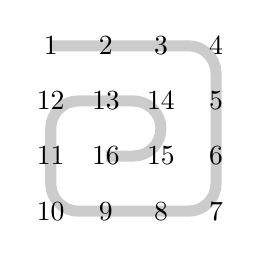
\begin{tikzpicture}[scale=0.7]
\def\stevilke{{7,8,9,10,6,1,2,11,5,4,3,-1}}
\draw [rounded corners=10pt,color=gray!40, line width=4pt]
(0, 0) -- (1, 0) -- (2, 0) -- (3, 0) -- (3, -1) -- (3, -2) -- (3, -3) -- (2, -3) -- (1, -3) -- (0, -3) --
(0, -2) -- (0, -1) -- (1, -1) -- (2, -1) -- (2, -2) -- (1, -2);
\node at (0, 0) {1};
\node at (1, 0) {2};
\node at (2, 0) {3};
\node at (3, 0) {4};
\node at (3, -1) {5};
\node at (3, -2) {6};
\node at (3, -3) {7};
\node at (2, -3) {8};
\node at (1, -3) {9};
\node at (0, -3) {10};
\node at (0, -2) {11};
\node at (0, -1) {12};
\node at (1, -1) {13};
\node at (2, -1) {14};
\node at (2, -2) {15};
\node at (1, -2) {16};
\end{tikzpicture}
$$

\noindent Matrika naj bo tako velika, kot je nujno potrebno, da lahko vanjo pospravimo celega polžka. Morebitna ``prazna polja'' zapolnimo z ničlami.  Zgled:
%
\begin{verbatim}
In[1]:= polzek[{1, 4, -1, -3, 2}]
Out[1]= {{1, 4, -1}, {0, 0, -3}, {0, 0, 2}}
In[2]:= polzek[{2, 3, 5, 7, 11, 13, 17, 19, 23, 29, 2, 7}]
Out[2]= {{2, 3, 5, 7}, {7, 0, 0, 11}, {2, 0, 0, 13}, {29, 23, 19, 17}}
\end{verbatim}

\podnaloga[10 točk]
V \emph{Mathematici} sestavite še ``inverzno'' funkcijo \texttt{odvij[m\_]}, ki kot argument dobi kvadratno matriko \texttt{m} ter vrne seznam elementov te matrike, tako da bo veljajo $$\texttt{polzek[odvij[m]] == m}.$$ Zgled:
%
\begin{verbatim}
In[3]:= odvij[{{1, 4, -1}, {0, 0, -3}, {0, 0, 2}}]
Out[3]= {1, 4, -1, -3, 2, 0, 0, 0, 0}
In[4]:= odvij[{{2, 3, 5, 7}, {7, 0, 0, 11}, {2, 0, 0, 13}, {29, 23, 19, 17}}]
Out[4]= {2, 3, 5, 7, 11, 13, 17, 19, 23, 29, 2, 7, 0, 0, 0, 0}
\end{verbatim}

%%%%%%%%%%%%%%%%%%%%%%%%%%%%%%%%%%%%%%%%%%%%%%%%%%%%%%%%%%%%%%%%%%%%%%
\naloga[Šestkotniki, 30 točk]

Znano je, da lahko ravnino tlakujemo s pravilnimi šestkotniki. Na tako dobljeni šestkotniški mreži vpeljemo koordinatni sistem, tako da vsak element iz $\mathbb{Z} \times \mathbb{Z}$ označuje natanko določen šestkotnik, kot je prikazano na skici:

$$
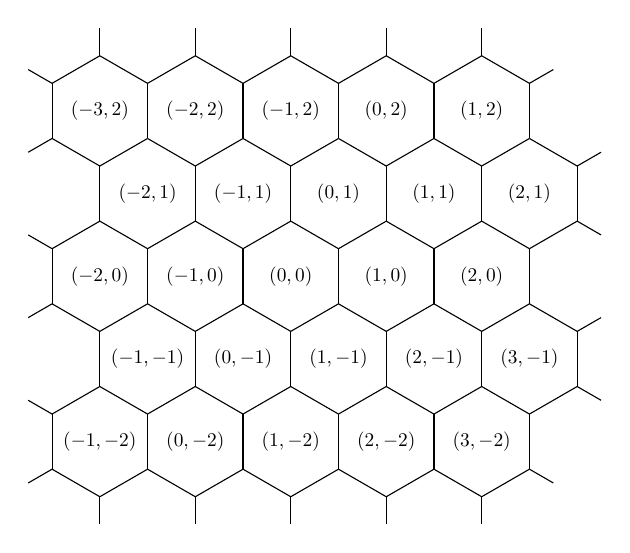
\begin{tikzpicture}[scale=0.7,  transform shape]
\tikzstyle{external coordinate} = []
\tikzstyle{internal coordinate} = []
\tikzstyle{hexalabel} = []
\tikzstyle{border coordinate} = []
\tikzstyle{internal hexagon} = []
\tikzstyle{external hexagon} = []
\tikzstyle{internal vertex} = [inner sep=2, draw, circle, fill=red]
\tikzstyle{border vertex} = [inner sep=2, draw, circle, fill=blue]
\tikzstyle{border edge} = [draw, color=black]
\tikzstyle{internal edge} = [draw, color=black]
\tikzstyle{external edge} = [draw, color=green]
\coordinate[border coordinate] (c_1) at (0.00000, 0.00000);
\coordinate[border coordinate] (c_2) at (0.86603, 0.50000);
\coordinate[border coordinate] (c_3) at (1.73205, 0.00000);
\coordinate[internal coordinate] (c_4) at (1.73205, -1.00000);
\coordinate[border coordinate] (c_5) at (0.86603, -1.50000);
\coordinate[border coordinate] (c_6) at (0.00000, -1.00000);
\coordinate[border coordinate] (c_7) at (2.59808, 0.50000);
\coordinate[border coordinate] (c_8) at (3.46410, 0.00000);
\coordinate[internal coordinate] (c_9) at (3.46410, -1.00000);
\coordinate[internal coordinate] (c_10) at (2.59808, -1.50000);
\coordinate[border coordinate] (c_11) at (4.33013, 0.50000);
\coordinate[border coordinate] (c_12) at (5.19615, 0.00000);
\coordinate[internal coordinate] (c_13) at (5.19615, -1.00000);
\coordinate[internal coordinate] (c_14) at (4.33013, -1.50000);
\coordinate[border coordinate] (c_15) at (6.06218, 0.50000);
\coordinate[border coordinate] (c_16) at (6.92820, 0.00000);
\coordinate[internal coordinate] (c_17) at (6.92820, -1.00000);
\coordinate[internal coordinate] (c_18) at (6.06218, -1.50000);
\coordinate[border coordinate] (c_19) at (7.79423, 0.50000);
\coordinate[border coordinate] (c_20) at (8.66025, 0.00000);
\coordinate[border coordinate] (c_21) at (8.66025, -1.00000);
\coordinate[internal coordinate] (c_22) at (7.79423, -1.50000);
\coordinate[internal coordinate] (c_23) at (2.59808, -2.50000);
\coordinate[internal coordinate] (c_24) at (1.73205, -3.00000);
\coordinate[border coordinate] (c_25) at (0.86603, -2.50000);
\coordinate[internal coordinate] (c_26) at (4.33013, -2.50000);
\coordinate[internal coordinate] (c_27) at (3.46410, -3.00000);
\coordinate[internal coordinate] (c_28) at (6.06218, -2.50000);
\coordinate[internal coordinate] (c_29) at (5.19615, -3.00000);
\coordinate[internal coordinate] (c_30) at (7.79423, -2.50000);
\coordinate[internal coordinate] (c_31) at (6.92820, -3.00000);
\coordinate[border coordinate] (c_32) at (9.52628, -1.50000);
\coordinate[border coordinate] (c_33) at (9.52628, -2.50000);
\coordinate[border coordinate] (c_34) at (8.66025, -3.00000);
\coordinate[border coordinate] (c_35) at (0.00000, -3.00000);
\coordinate[internal coordinate] (c_36) at (1.73205, -4.00000);
\coordinate[border coordinate] (c_37) at (0.86603, -4.50000);
\coordinate[border coordinate] (c_38) at (0.00000, -4.00000);
\coordinate[internal coordinate] (c_39) at (3.46410, -4.00000);
\coordinate[internal coordinate] (c_40) at (2.59808, -4.50000);
\coordinate[internal coordinate] (c_41) at (5.19615, -4.00000);
\coordinate[internal coordinate] (c_42) at (4.33013, -4.50000);
\coordinate[internal coordinate] (c_43) at (6.92820, -4.00000);
\coordinate[internal coordinate] (c_44) at (6.06218, -4.50000);
\coordinate[border coordinate] (c_45) at (8.66025, -4.00000);
\coordinate[internal coordinate] (c_46) at (7.79423, -4.50000);
\coordinate[internal coordinate] (c_47) at (2.59808, -5.50000);
\coordinate[internal coordinate] (c_48) at (1.73205, -6.00000);
\coordinate[border coordinate] (c_49) at (0.86603, -5.50000);
\coordinate[internal coordinate] (c_50) at (4.33013, -5.50000);
\coordinate[internal coordinate] (c_51) at (3.46410, -6.00000);
\coordinate[internal coordinate] (c_52) at (6.06218, -5.50000);
\coordinate[internal coordinate] (c_53) at (5.19615, -6.00000);
\coordinate[internal coordinate] (c_54) at (7.79423, -5.50000);
\coordinate[internal coordinate] (c_55) at (6.92820, -6.00000);
\coordinate[border coordinate] (c_56) at (9.52628, -4.50000);
\coordinate[border coordinate] (c_57) at (9.52628, -5.50000);
\coordinate[border coordinate] (c_58) at (8.66025, -6.00000);
\coordinate[border coordinate] (c_59) at (0.00000, -6.00000);
\coordinate[border coordinate] (c_60) at (1.73205, -7.00000);
\coordinate[border coordinate] (c_61) at (0.86603, -7.50000);
\coordinate[border coordinate] (c_62) at (0.00000, -7.00000);
\coordinate[border coordinate] (c_63) at (3.46410, -7.00000);
\coordinate[border coordinate] (c_64) at (2.59808, -7.50000);
\coordinate[border coordinate] (c_65) at (5.19615, -7.00000);
\coordinate[border coordinate] (c_66) at (4.33013, -7.50000);
\coordinate[border coordinate] (c_67) at (6.92820, -7.00000);
\coordinate[border coordinate] (c_68) at (6.06218, -7.50000);
\coordinate[border coordinate] (c_69) at (8.66025, -7.00000);
\coordinate[border coordinate] (c_70) at (7.79423, -7.50000);
\path[internal hexagon] (c_1) -- (c_2) -- (c_3) -- (c_4) -- (c_5) -- (c_6) -- cycle;
\node[hexalabel] at (0.86603, -0.50000) {$(-3, 2)$};
\path[internal hexagon] (c_3) -- (c_7) -- (c_8) -- (c_9) -- (c_10) -- (c_4) -- cycle;
\node[hexalabel] at (2.59808, -0.50000) {$(-2, 2)$};
\path[internal hexagon] (c_8) -- (c_11) -- (c_12) -- (c_13) -- (c_14) -- (c_9) -- cycle;
\node[hexalabel] at (4.33013, -0.50000) {$(-1, 2)$};
\path[internal hexagon] (c_12) -- (c_15) -- (c_16) -- (c_17) -- (c_18) -- (c_13) -- cycle;
\node[hexalabel] at (6.06218, -0.50000) {$(0, 2)$};
\path[internal hexagon] (c_16) -- (c_19) -- (c_20) -- (c_21) -- (c_22) -- (c_17) -- cycle;
\node[hexalabel] at (7.79423, -0.50000) {$(1, 2)$};
\path[internal hexagon] (c_5) -- (c_4) -- (c_10) -- (c_23) -- (c_24) -- (c_25) -- cycle;
\node[hexalabel] at (1.73205, -2.00000) {$(-2, 1)$};
\path[internal hexagon] (c_10) -- (c_9) -- (c_14) -- (c_26) -- (c_27) -- (c_23) -- cycle;
\node[hexalabel] at (3.46410, -2.00000) {$(-1, 1)$};
\path[internal hexagon] (c_14) -- (c_13) -- (c_18) -- (c_28) -- (c_29) -- (c_26) -- cycle;
\node[hexalabel] at (5.19615, -2.00000) {$(0, 1)$};
\path[internal hexagon] (c_18) -- (c_17) -- (c_22) -- (c_30) -- (c_31) -- (c_28) -- cycle;
\node[hexalabel] at (6.92820, -2.00000) {$(1, 1)$};
\path[internal hexagon] (c_22) -- (c_21) -- (c_32) -- (c_33) -- (c_34) -- (c_30) -- cycle;
\node[hexalabel] at (8.66025, -2.00000) {$(2, 1)$};
\path[internal hexagon] (c_35) -- (c_25) -- (c_24) -- (c_36) -- (c_37) -- (c_38) -- cycle;
\node[hexalabel] at (0.86603, -3.50000) {$(-2, 0)$};
\path[internal hexagon] (c_24) -- (c_23) -- (c_27) -- (c_39) -- (c_40) -- (c_36) -- cycle;
\node[hexalabel] at (2.59808, -3.50000) {$(-1, 0)$};
\path[internal hexagon] (c_27) -- (c_26) -- (c_29) -- (c_41) -- (c_42) -- (c_39) -- cycle;
\node[hexalabel] at (4.33013, -3.50000) {$(0, 0)$};
\path[internal hexagon] (c_29) -- (c_28) -- (c_31) -- (c_43) -- (c_44) -- (c_41) -- cycle;
\node[hexalabel] at (6.06218, -3.50000) {$(1, 0)$};
\path[internal hexagon] (c_31) -- (c_30) -- (c_34) -- (c_45) -- (c_46) -- (c_43) -- cycle;
\node[hexalabel] at (7.79423, -3.50000) {$(2, 0)$};
\path[internal hexagon] (c_37) -- (c_36) -- (c_40) -- (c_47) -- (c_48) -- (c_49) -- cycle;
\node[hexalabel] at (1.73205, -5.00000) {$(-1, -1)$};
\path[internal hexagon] (c_40) -- (c_39) -- (c_42) -- (c_50) -- (c_51) -- (c_47) -- cycle;
\node[hexalabel] at (3.46410, -5.00000) {$(0, -1)$};
\path[internal hexagon] (c_42) -- (c_41) -- (c_44) -- (c_52) -- (c_53) -- (c_50) -- cycle;
\node[hexalabel] at (5.19615, -5.00000) {$(1, -1)$};
\path[internal hexagon] (c_44) -- (c_43) -- (c_46) -- (c_54) -- (c_55) -- (c_52) -- cycle;
\node[hexalabel] at (6.92820, -5.00000) {$(2, -1)$};
\path[internal hexagon] (c_46) -- (c_45) -- (c_56) -- (c_57) -- (c_58) -- (c_54) -- cycle;
\node[hexalabel] at (8.66025, -5.00000) {$(3, -1)$};
\path[internal hexagon] (c_59) -- (c_49) -- (c_48) -- (c_60) -- (c_61) -- (c_62) -- cycle;
\node[hexalabel] at (0.86603, -6.50000) {$(-1, -2)$};
\path[internal hexagon] (c_48) -- (c_47) -- (c_51) -- (c_63) -- (c_64) -- (c_60) -- cycle;
\node[hexalabel] at (2.59808, -6.50000) {$(0, -2)$};
\path[internal hexagon] (c_51) -- (c_50) -- (c_53) -- (c_65) -- (c_66) -- (c_63) -- cycle;
\node[hexalabel] at (4.33013, -6.50000) {$(1, -2)$};
\path[internal hexagon] (c_53) -- (c_52) -- (c_55) -- (c_67) -- (c_68) -- (c_65) -- cycle;
\node[hexalabel] at (6.06218, -6.50000) {$(2, -2)$};
\path[internal hexagon] (c_55) -- (c_54) -- (c_58) -- (c_69) -- (c_70) -- (c_67) -- cycle;
\node[hexalabel] at (7.79423, -6.50000) {$(3, -2)$};
%
% \path[draw] (9.5, -0.50000) -- (11, -0.50000);
% \node[hexalabel] at ({11+0.7}, -0.50000) {$\eta = 2$};
% \path[draw] (10.5, -2.0000) -- (12, -2.0000);
% \node[hexalabel] at ({12+0.7}, -2.00000) {$\eta = 1$};
% \path[draw] (9.5, -3.50000) -- (11, -3.50000);
% \node[hexalabel] at ({11+0.7}, -3.50000) {$\eta = 0$};
% \path[draw] (10.5, -5.0000) -- (12, -5.0000);
% \node[hexalabel] at ({12+0.9}, -5.00000) {$\eta = -1$};
% \path[draw] (9.5, -6.5000) -- (11, -6.5000);
% \node[hexalabel] at ({11+0.9}, -6.50000) {$\eta = -2$};
%
% \path[draw] (7.79423 + 0.8*-0.86602, -6.50000 + 0.8*-1.5) -- ({7.79423 + 1.5*-0.86602}, {-6.50000 + 1.5*-1.5});
% \node[hexalabel, rotate=60] at ({7.79423 + 1.9*-0.86602}, {-6.50000 + 1.9*-1.5}) {$\xi = 3$};
% \path[draw] (6.06218 + 0.8*-0.86602, -6.50000 + 0.8*-1.5) -- ({6.06218 + 1.5*-0.86602}, {-6.50000 + 1.5*-1.5});
% \node[hexalabel, rotate=60] at ({6.06218 + 1.9*-0.86602}, {-6.50000 + 1.9*-1.5}) {$\xi = 2$};
% \path[draw] (4.33013 + 0.8*-0.86602, -6.50000 + 0.8*-1.5) -- ({4.33013 + 1.5*-0.86602}, {-6.50000 + 1.5*-1.5});
% \node[hexalabel, rotate=60] at ({4.33013 + 1.9*-0.86602}, {-6.50000 + 1.9*-1.5}) {$\xi = 1$};
% \path[draw] (2.59808 + 0.8*-0.86602, -6.50000 + 0.8*-1.5) -- ({2.59808 + 1.5*-0.86602}, {-6.50000 + 1.5*-1.5});
% \node[hexalabel, rotate=60] at ({2.59808 + 1.9*-0.86602}, {-6.50000 + 1.9*-1.5}) {$\xi = 0$};
% \path[draw] (0.86603 + 0.8*-0.86602, -6.50000 + 0.8*-1.5) -- ({0.86603 + 1.5*-0.86602}, {-6.50000 + 1.5*-1.5});
% \node[hexalabel, rotate=60] at ({0.86603 + 2*-0.86602}, {-6.50000 + 2*-1.5}) {$\xi = -1$};
%
% \path[draw] (7.79423 + 0.8*-0.86602, -0.50000 + 0.8*1.5) -- ({7.79423 + 1.5*-0.86602}, {-0.50000 + 1.5*1.5});
% \node[hexalabel, rotate=-60] at ({7.79423 + 1.9*-0.86602}, {-0.50000 + 1.9*1.5}) {$\zeta = 3$};
% \path[draw] (6.06218 + 0.8*-0.86602, -0.50000 + 0.8*1.5) -- ({6.06218 + 1.5*-0.86602}, {-0.50000 + 1.5*1.5});
% \node[hexalabel, rotate=-60] at ({6.06218 + 1.9*-0.86602}, {-0.50000 + 1.9*1.5}) {$\zeta = 2$};
% \path[draw] (4.33013 + 0.8*-0.86602, -0.50000 + 0.8*1.5) -- ({4.33013 + 1.5*-0.86602}, {-0.50000 + 1.5*1.5});
% \node[hexalabel, rotate=-60] at ({4.33013 + 1.9*-0.86602}, {-0.50000 + 1.9*1.5}) {$\zeta = 1$};
% \path[draw] (2.59808 + 0.8*-0.86602, -0.50000 + 0.8*1.5) -- ({2.59808 + 1.5*-0.86602}, {-0.50000 + 1.5*1.5});
% \node[hexalabel, rotate=-60] at ({2.59808 + 1.9*-0.86602}, {-0.50000 + 1.9*1.5}) {$\zeta = 0$};
% \path[draw] (0.86603 + 0.8*-0.86602, -0.50000 + 0.8*1.5) -- ({0.86603 + 1.5*-0.86602}, {-0.50000 + 1.5*1.5});
% \node[hexalabel, rotate=-60] at ({0.86603 + 2*-0.86602}, {-0.50000 + 2*1.5}) {$\zeta = -1$};
%
\path[border edge] (c_1) -- (c_2);
\path[border edge] (c_2) -- (c_3);
\path[internal edge] (c_3) -- (c_4);
\path[internal edge] (c_4) -- (c_5);
\path[border edge] (c_5) -- (c_6);
\path[border edge] (c_6) -- (c_1);
\path[border edge] (c_3) -- (c_7);
\path[border edge] (c_7) -- (c_8);
\path[internal edge] (c_8) -- (c_9);
\path[internal edge] (c_9) -- (c_10);
\path[internal edge] (c_10) -- (c_4);
\path[border edge] (c_8) -- (c_11);
\path[border edge] (c_11) -- (c_12);
\path[internal edge] (c_12) -- (c_13);
\path[internal edge] (c_13) -- (c_14);
\path[internal edge] (c_14) -- (c_9);
\path[border edge] (c_12) -- (c_15);
\path[border edge] (c_15) -- (c_16);
\path[internal edge] (c_16) -- (c_17);
\path[internal edge] (c_17) -- (c_18);
\path[internal edge] (c_18) -- (c_13);
\path[border edge] (c_16) -- (c_19);
\path[border edge] (c_19) -- (c_20);
\path[border edge] (c_20) -- (c_21);
\path[internal edge] (c_21) -- (c_22);
\path[internal edge] (c_22) -- (c_17);
\path[internal edge] (c_10) -- (c_23);
\path[internal edge] (c_23) -- (c_24);
\path[internal edge] (c_24) -- (c_25);
\path[border edge] (c_25) -- (c_5);
\path[internal edge] (c_14) -- (c_26);
\path[internal edge] (c_26) -- (c_27);
\path[internal edge] (c_27) -- (c_23);
\path[internal edge] (c_18) -- (c_28);
\path[internal edge] (c_28) -- (c_29);
\path[internal edge] (c_29) -- (c_26);
\path[internal edge] (c_22) -- (c_30);
\path[internal edge] (c_30) -- (c_31);
\path[internal edge] (c_31) -- (c_28);
\path[border edge] (c_21) -- (c_32);
\path[border edge] (c_32) -- (c_33);
\path[border edge] (c_33) -- (c_34);
\path[internal edge] (c_34) -- (c_30);
\path[border edge] (c_35) -- (c_25);
\path[internal edge] (c_24) -- (c_36);
\path[internal edge] (c_36) -- (c_37);
\path[border edge] (c_37) -- (c_38);
\path[border edge] (c_38) -- (c_35);
\path[internal edge] (c_27) -- (c_39);
\path[internal edge] (c_39) -- (c_40);
\path[internal edge] (c_40) -- (c_36);
\path[internal edge] (c_29) -- (c_41);
\path[internal edge] (c_41) -- (c_42);
\path[internal edge] (c_42) -- (c_39);
\path[internal edge] (c_31) -- (c_43);
\path[internal edge] (c_43) -- (c_44);
\path[internal edge] (c_44) -- (c_41);
\path[border edge] (c_34) -- (c_45);
\path[internal edge] (c_45) -- (c_46);
\path[internal edge] (c_46) -- (c_43);
\path[internal edge] (c_40) -- (c_47);
\path[internal edge] (c_47) -- (c_48);
\path[internal edge] (c_48) -- (c_49);
\path[border edge] (c_49) -- (c_37);
\path[internal edge] (c_42) -- (c_50);
\path[internal edge] (c_50) -- (c_51);
\path[internal edge] (c_51) -- (c_47);
\path[internal edge] (c_44) -- (c_52);
\path[internal edge] (c_52) -- (c_53);
\path[internal edge] (c_53) -- (c_50);
\path[internal edge] (c_46) -- (c_54);
\path[internal edge] (c_54) -- (c_55);
\path[internal edge] (c_55) -- (c_52);
\path[border edge] (c_45) -- (c_56);
\path[border edge] (c_56) -- (c_57);
\path[border edge] (c_57) -- (c_58);
\path[internal edge] (c_58) -- (c_54);
\path[border edge] (c_59) -- (c_49);
\path[internal edge] (c_48) -- (c_60);
\path[border edge] (c_60) -- (c_61);
\path[border edge] (c_61) -- (c_62);
\path[border edge] (c_62) -- (c_59);
\path[internal edge] (c_51) -- (c_63);
\path[border edge] (c_63) -- (c_64);
\path[border edge] (c_64) -- (c_60);
\path[internal edge] (c_53) -- (c_65);
\path[border edge] (c_65) -- (c_66);
\path[border edge] (c_66) -- (c_63);
\path[internal edge] (c_55) -- (c_67);
\path[border edge] (c_67) -- (c_68);
\path[border edge] (c_68) -- (c_65);
\path[border edge] (c_58) -- (c_69);
\path[border edge] (c_69) -- (c_70);
\path[border edge] (c_70) -- (c_67);
\path[border edge] (c_70) -- ++(-90:0.5);
\path[border edge] (c_69) -- ++(-30:0.5);
\path[border edge] (c_68) -- ++(-90:0.5);
\path[border edge] (c_66) -- ++(-90:0.5);
\path[border edge] (c_64) -- ++(-90:0.5);
\path[border edge] (c_62) -- ++(-150:0.5);
\path[border edge] (c_61) -- ++(-90:0.5);
\path[border edge] (c_59) -- ++(150:0.5);
\path[border edge] (c_57) -- ++(-30:0.5);
\path[border edge] (c_56) -- ++(30:0.5);
\path[border edge] (c_38) -- ++(-150:0.5);
\path[border edge] (c_35) -- ++(150:0.5);
\path[border edge] (c_33) -- ++(-30:0.5);
\path[border edge] (c_32) -- ++(30:0.5);
\path[border edge] (c_7) -- ++(90:0.5);
\path[border edge] (c_6) -- ++(-150:0.5);
\path[border edge] (c_2) -- ++(90:0.5);
\path[border edge] (c_1) -- ++(150:0.5);
\path[border edge] (c_15) -- ++(90:0.5);
\path[border edge] (c_11) -- ++(90:0.5);
\path[border edge] (c_19) -- ++(90:0.5);
\path[border edge] (c_20) -- ++(30:0.5);
\end{tikzpicture}

$$

\noindent V \emph{Mathematici} sestavite funkcijo \texttt{benz[l\_]}, ki kot argument dobi seznam \texttt{l} in nariše tiste šest\-kot\-nike, ki so podani v seznamu \texttt{l}. Šestkotniki so podani z zgoraj opisanimi koordinatami, tj. kot pari celih števil (glejte zgornjo skico). Zgledi:

\vspace{\baselineskip}

\begin{center}
\begin{tabular}{c@{\hspace{1.5cm}}c}
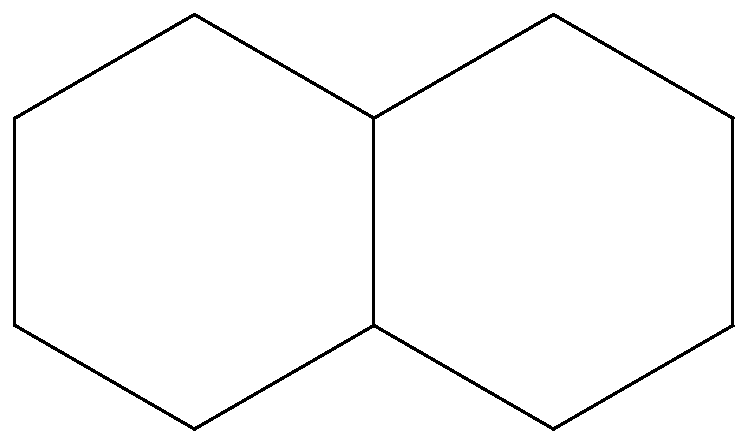
\includegraphics[scale=0.35]{hex01.pdf} & 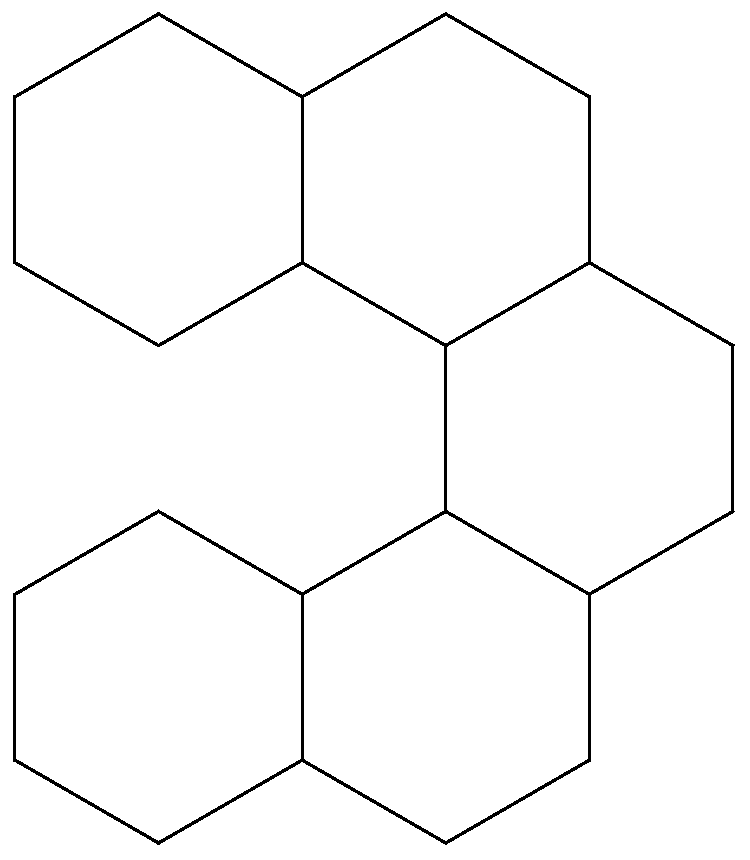
\includegraphics[scale=0.4]{hex02.pdf}\\
\texttt{benz[\{\{-1, 0\}, \{0, 0\}\}]} &   \texttt{benz[\{\{0, 0\}, \{1, 0\}, \{1, 1\}, \{0, 2\}, \{-1, 2\}\}]}
\end{tabular}
\end{center}

\vspace{\baselineskip}

\noindent \emph{Namig:} Pravokotni koordinatni sistem postavimo tako, da je izhodišče koordinatnega sistema v središču šestkotnika z oznako $(0, 0)$. Katera točka je središče šestkotnika z oznako $(u, v)$?


%%%%%%%%%%%%%%%%%%%%%%%%%%%%%%%%%%%%%%%%%%%%%%%%%%%%%%%%%%%%%%%%%%%%%%
\naloga[Dvojiško drevo, 10 + 10 + 10 točk]

Podatkovna struktura \texttt{Drevo} predstavlja dvojiško drevo, ki ima v vsakem vozlišču shranjeno eno celo število. Naslednji izraz v Pythonu ustvari drevo, ki je prikazano na spodnji sliki:
%
\begin{verbatim}
  >>> s = Drevo(20, levo=Drevo(3, levo=Drevo(3)), desno=Drevo(7, levo=Drevo(7),
          desno=Drevo(0, levo=Drevo(-5), desno=Drevo(5))))
\end{verbatim}

\noindent Pripadajoča slika:
\vspace{-0.4cm}
\begin{center}
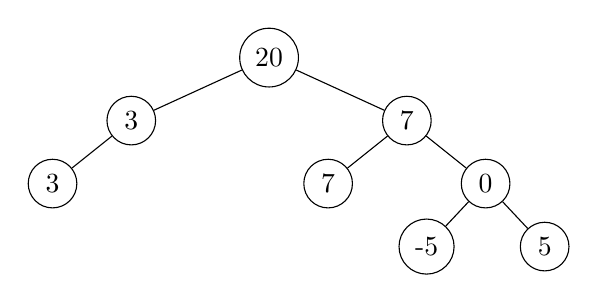
\begin{tikzpicture}[level distance=0.8cm,
    level 1/.style={sibling distance=3.5cm},
    level 2/.style={sibling distance=2cm},
    level 3/.style={sibling distance=1.5cm}
    ]
    \node[circle, draw] (d) {20}
      child {node[circle, draw] {3}
        child {node[circle, draw] {3}}
        child[missing] {}
      }
      child {node[circle, draw] {7}
        child {node[circle, draw] {7}}
        child {node[circle, draw] {0}
          child {node[circle, draw] {-5}}
          child {node[circle, draw] {5}}
        }
      };
  \end{tikzpicture}
\end{center}
%
Rekli bomo, da je drevo \emph{sumarno}, če za vsako vozlišče, ki ni list, velja, da je njegova vrednost enaka vsoti vseh števil, ki so pod njim (tj.\ v levem in v desnem poddrevesu). Zgornje drevo je primer sumarnega drevesa.

Razred \texttt{Drevo} je že delno implementiran. Vsako vozlišče ima atribut \texttt{prazno}. Če je njegova vrednost \texttt{True}, predstavlja prazno poddrevo in nima drugih atributov. Če pa drevo ni prazno, ima še atribute \texttt{vsebina}, \texttt{levo} in \texttt{desno}. Dodali bomo še nekaj novih metod.
%
\podnaloga[10 točk]
%
Razredu \texttt{Drevo} dodajte metodo \texttt{je\_sumarno(self)}, ki vrne \texttt{True}, če je drevo sumarno, in \texttt{False} sicer. Za prazno drevo naj metoda tudi vrne \texttt{True}.
Zgledi:
%
\begin{verbatim}
  >>> s.je_sumarno()
  True
  >>> Drevo(3, levo=Drevo(1), desno=Drevo(1)).je_sumarno()
  False
\end{verbatim}
%
\podnaloga[10 točk]
%
Izkaže se, da so vse vrednosti v sumarnem drevesu enolično določene takoj, ko podamo vrednosti v listih. Razredu \texttt{Drevo} dodajte metodo \texttt{naredi\_sumarno(self)}, ki drevo popravi, tako da le-to postane sumarno. Vrednosti v listih metoda ne sme spreminjati. Zgled:
%
\begin{verbatim}
  >>> d = Drevo(3, levo=Drevo(1), desno=Drevo(1))
  >>> d.naredi_sumarno()
  >>> d
  Drevo(2, levo=Drevo(1), desno=Drevo(1))
\end{verbatim}
%

\podnaloga[10 točk]
%
Razredu \texttt{Drevo} dodajte metodo \texttt{pristej\_po\_poti(self, x, p)}, ki kot argument dobi število \texttt{x} in seznam \texttt{p}. Začnemo v korenu drevesa in gremo po poti, tako da se vsakič spustimo v eno od poddreves. Elementi seznama \texttt{p} nam povedo, v katero poddrevo se spustimo: niz \texttt{'l'} pomeni, da gremo v levo poddrevo; niz \texttt{'d'} pomeni, da gremo v desno poddrevo. Ko pridemo do praznega poddrevesa, se ustavimo. Če v seznamu \texttt{p} zmanja elementov, začnemo spet pri začetku (kakor da bi bil seznam \texttt{p} cikličen). Drevo pri tem spremenimo tako, da vsem elementom na tej poti prištejemo število \texttt{x}. Primer:
\begin{verbatim}
  >>> s.pristej_po_poti(2, ['d', 'l', 'd'])
  >>> s
  Drevo(22, levo=Drevo(3, levo=Drevo(3)), desno=Drevo(9, levo=Drevo(9),
  desno=Drevo(0, levo=Drevo(-5), desno=Drevo(5))))
\end{verbatim}

\noindent Pripadajoča slika:
\vspace{-0.4cm}
\begin{center}
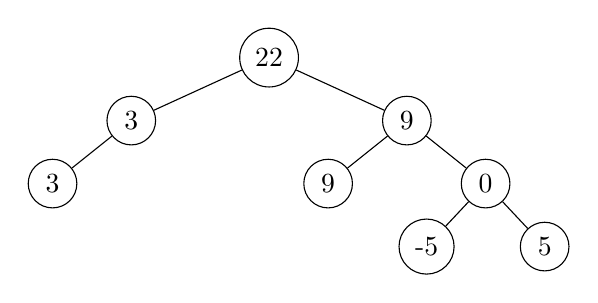
\begin{tikzpicture}[level distance=0.8cm,
    level 1/.style={sibling distance=3.5cm},
    level 2/.style={sibling distance=2cm},
    level 3/.style={sibling distance=1.5cm}
    ]
    \node[circle, draw] (d) {22}
      child {node[circle, draw] {3}
        child {node[circle, draw] {3}}
        child[missing] {}
      }
      child {node[circle, draw] {9}
        child {node[circle, draw] {9}}
        child {node[circle, draw] {0}
          child {node[circle, draw] {-5}}
          child {node[circle, draw] {5}}
        }
      };
  \end{tikzpicture}
\end{center}




%%%%%%%%%%%%%%%%%%%%%%%%%%%%%%%%%%%%%%%%%%%%%%%%%%%%%%%%%%%%%%%%%%%%%%
\naloga[Igra urejanja, 10 + 10 + 10 točk]

Mojca in Gorazd se igrata zanimivo igro, ki ji pravita \emph{Igra urejanja}. Začneta z nekim seznamom $\ell$ dolžine $n$, ki vsebuje vsa števila med 0 in $n-1$, na primer
$$
\ell = [0, 3, 6, 7, 8, 4, 5, 1, 2].
$$
Začne Gorazd, ki lahko v eni potezi  med seboj zamenja poljubna dva elementa seznama. Poteza
$(1, 5)$ pomeni, da med seboj zamenja 1.\ in 5.\ element. Iz gornjega seznama bi tako dobil:
$$
[0, 4, 6, 7, 8, 3, 5, 1, 2].
$$
Mojca po vsaki Gorazdovi potezi lahko reče ``Dalje!'' ali pa ``Stop!''. Če reče ``Dalje!'', Gorazd nadaljuje s svojo naslednjo potezo. Če Mojca reče ``Stop!'', Gorazd prekine z izvajanjem svojih potez. Mojca pa mora seznam $\ell$ urediti naraščajoče, pri čemer sme porabiti največ toliko potez, kot jih je do tega trenutka naredil Gorazd. Če Mojci ne uspe urediti seznama, izgubi partijo.

\podnaloga[10 točk]
Mojca je opazila, da seznam $\ell$ pravzaprav predstavlja permutacijo $i \mapsto \ell[i]$ na množici \{0, 1, \ldots, n-1\}. Sestavite funkcijo \texttt{ciklicni\_zapis(l)}, ki vrne ciklični zapis permutacije, ki je podana s seznamom \texttt{l}. Cikli naj bodo urejeni leksikografsko, na prvem mestu v vsakem ciklu pa naj bo najmanjši element. Zgled:

\begin{verbatim}
  >>> ciklicni_zapis([0, 3, 6, 7, 8, 4, 5, 1, 2])
  [[0], [1, 3, 7], [2, 6, 5, 4, 8]]
\end{verbatim}

\noindent 

\podnaloga[10 točk]
Mojca je ugotovila, da je vsaka Gorazdova poteza v bistvu množenje z leve z ustrezno transpozicijo. V gornjem primeru to pomeni
$$
(1\ 5) * (0)\ (1\ 3\ 7)\ (2\ 6\ 5\ 4\ 8) = (0)\ (1\ 4\ 8\ 2\ 6\ 5\ 3\ 7).
$$
Mojca je ugotovila še, da lahko z eno transpozicijo:
\begin{compactitem}
\item združimo dva cikla v enega ali pa
\item en cikel razbijemo na dva manjša.
\end{compactitem}
Ker urejen seznam ustreza identični permutaciji, moramo vse cikle razbiti do ciklov dolžine 1.
Minimalno število potez, ki jih za to potrebujemo, lahko preberemo iz cikličnega tipa permutacije (za razbijanje cikla dolžine $d$ potrebujemo $d-1$ transpozicij).

Sestavite funkcijo \texttt{razbij\_cikle(p)}, ki kot argument dobi permutacijo \texttt{p}, ki je podana s cikličnim zapisom. Funkcija naj vrne seznam transpozicij, s katerimi moramo (z leve) pomnožiti permutacijo \texttt{p}, da dobimo identiteto. Število teh transpozicij mora biti najmanjše možno. Zgled:

\begin{verbatim}
  >>> razbij_cikle([[0, 4, 3], [1, 5], [2], [7, 8, 9, 6]])
  [(0, 4), (0, 3), (1, 5), (7, 8), (7, 9), (7, 6)]
\end{verbatim}

\noindent \emph{Opomba:} Tomo bo sprejel vse pravilne rešitve, tudi če vaša funkcija vrne rezultat, ki se razlikuje od ``uradnega''.

\podnaloga[10 točk]
Prej ko Mojca reče ``Stop!'', več točk bo dobila. Če lahko Mojca seznam uredi po $k$ Gorazdovih potezah, ga lahko uredi tudi po $k + 1$ potezah (npr. tako, da razveljavi zadnjo njegovo potezo in postopa enako, kot bi tudi sicer po $k$-ti njegovi potezi). To pomeni, da lahko minimalno število potez, ki jih potrebuje za zmago, poišče z bisekcijo.

\emph{Napotek:} Po tem, ko Gorazd na seznamu izvede $k$ zamenjav, Mojca poišče ciklični zapis ter pogleda, če za razbijanje ciklov res porabi kvečjemu $k$ transpozicij.

Napišite funkcijo \texttt{min\_potez(l, g)}, ki kot argumenta dobi začetni seznam \texttt{l} in seznam trans\-pozicij \texttt{g}, ki jih bo izvedel Gorazd. Funkcija naj vrne najmanjše število potez, ki jih izvede Gorazd, preden ima Mojca prvo priložnost za zmago. Gorazd poteze dela dovolj dolgo časa, da ima Mojca možnost za zmago. Če je seznam \texttt{l} že na začetku urejen, lahko Mojca zavpije ``Stop!'', še preden Gorazd naredi prvo potezo. Zgled:

\begin{verbatim}
  >>> min_potez([0, 3, 6, 7, 8, 4, 5, 1, 2],
                [(1, 5), (1, 2), (4, 5), (7, 8), (2, 3), (1, 6), (3, 7)])
  5
\end{verbatim}

\end{document}
